\documentclass[12pt]{article}
\usepackage{xeCJK}
\usepackage{amsmath}
\usepackage{pdfpages}
\usepackage[colorlinks,linkcolor=red]{hyperref}

\title{Project 2}
\author{
李林翼 \footnote{计43, 2014011361, limyik.li96@gmail.com}
\ 朱祺 \footnote{计43, 2014011336, zhu-q14@mails.tsinghua.edu.cn}
}
\begin{document}
\maketitle{}
\tableofcontents
\newpage

\section{引言}
\subsection{实验环境}
使用Python语言编写,版本2.7.10,使用的工具包有:
\begin{description}
  \item[ElementTree]
  预处理时用于解析xml格式的新闻
  \item[enchant]
  预处理时用于拼写检查
  \item[nltk]
  预处理时用于分词,词干化等自然语言处理
  \item[numpy]
  \item[sklearn]
  \item[xgboost]
  Gradient Boost
  \item[matplotlib]
  可视化
\end{description}
\subsection{分工}
\begin{tabular}{l|c|c|c|c|c}
  \hline
   &预处理&分类&ensemble&聚类&可视化\\
  \hline
  李林翼&${\surd}$&基本&bootstrap,adaboost,random forest& &\\
  \hline
  朱祺&&knn,lda&xgboost, bagging(kNN)&基本&${\surd}$\\
  \hline
\end{tabular}

\section{数据预处理和特征提取}
\subsection{新闻数据读入}
抽取 docid, categories, full-text 属性,这部分与 project 1 类似。每篇文档可能有多个类别。
同时,提取出出现次数大于500次的类别,作为分类时的类别,有26个类。去除没有类别标签或没有全文的。
\subsection{对全文进行预处理}
使用enchant、nltk自然语言处理的工具包,对新闻全文依次进行以下处理:分句、分词、拼写检查、
去除短词与停用词、词干化、去除短词与停用词。之后,得到词袋模型。
\subsection{转化成tfidf向量}
从词袋模型得到字典,包含出现次数大于10的词。利用词袋模型和字典,
将每篇文档用tfidf的向量表示,得到(48793, 24541)的矩阵,即48793篇文档,字典大小24541。同时,
所有新闻按照9:1的比例随机分成训练集和测试集。
\subsection{降维}
鉴于上一步得到的tfidf向量维度太大了,不利于保存和分类,因此使用pca降维到100维。为了后面将要进行的
聚类可视化任务,也用pca降到2维。

\section{基本分类器的运用和比较}
使用的分类算法除了要求的 Logistic Regression, Naive Bayes, SVM, Decision Tree, MLP, 还有
k Nearest Neighbors, Linear Discriminant Analysis。这些算法 sklearn 中都有提供,其中
Naive Bayes 用的是高斯分布的 GaussianNB。\\
\\
10折,选择2号作为测试集。这些算法的训练集大小(43913, 100),测试集(4880, 100),这里将pca降维后
的数据进一步处理,使用 StandardScaler 标准化,移去均值缩放到单位方差。
共有26个类别,由于每篇文档可能有多个类别,因此对每个类训练一个二分类器,
用 sklearn 中 OneVsRestClassifier 方法辅助,完整的结果见result/log.txt。
\subsection{总体情况}
下面是 Pecision, Recall, F1-score 的\textbf{平均值},以及训练时间:\\
\\
\begin{tabular}{l|r|r|r|r}
  \hline
  平均值 &Pecision&Recall&F1-score&训练时间(s)\\
  \hline
  Logistic Regression& 0.72&0.45&0.53&84.3\\
  \hline
  Gaussian Naive Bayes&0.19&0.91&0.28& 1.7\\
  \hline
  SVM(SVC)&0.82&0.51&0.58& 1022.1\\
  \hline
  Decision Tree&0.59&0.61&0.60& 177.9\\
  \hline
  MLP&0.76&0.70&0.73& 658.6\\
  \hline
  kNN(k=5)&0.75&0.62&0.67& 7.9\\
  \hline
  Linear Discriminant Analysis&0.63&0.43&0.49& 22.3\\
  \hline
\end{tabular}
\\
\\
总体上来说,MLP 是效果最好的,但是训练时间较长。kNN 效果次之,训练时间短,但是预测的时间长,这与它
本身的特点有关。Decision Tree 的 Pecision 和 Recall 较接近,虽然两者都不高,但是F1-score还不错。
Linear Discriminant Analysis, Logistic Regression, SVM(SVC) 这三者比较相似,都是线性模型,
效果一个比一个好,但是训练时间也变长了,SVM(SVC) 的训练时间非常长。Gaussian Naive Bayes 效果很差,
可能数据分布不符合高斯的假设。
\\
\subsection{特定类别}
观察到不同类别的分类效果相差很大,比如对 paid death notices 类,每个分类器的分类效果都很好,而对
 travel 类等,线性模型如 Logistic Regression, SVM(SVC), Linear Discriminant Analysis 等
效果都很差(F1-score无法计算或接近0)。因此平均值不能完全反应分类器的效果,下面选择三个类别,比较在
这三个类别上分类器的表现。选择的是在各分类器中效果几乎都是最好的两个类,和在某些模型中很差,在另一些
模型中较好的一个类。\\
\\
\begin{tabular}{l|r|r|r}
  \hline
  类别:\textbf{paid death notices} &Pecision&Recall&F1-score\\
  \hline
  Logistic Regression& 0.99&0.98&0.98\\
  \hline
  Gaussian Naive Bayes&0.77&0.87&0.82\\
  \hline
  SVM(SVC)&0.98&0.99&0.99\\
  \hline
  Decision Tree&0.97&0.99&0.98\\
  \hline
  MLP&0.99&0.99&0.99\\
  \hline
  kNN(k=5)&1.00&0.85&0.91\\
  \hline
  Linear Discriminant Analysis&1.00&0.92&0.95\\
  \hline
\end{tabular}
\\
\\
paid death notices 类比较明显,各个分类器都有比较好的效果(除了 Gaussian Naive Bayes)。其中
Logistic Regression, SVM(SVC), Decision Tree, MLP 效果非常好,说明了数据本身对分类效果有
很大影响。
\\
\\
\begin{tabular}{l|r|r|r}
  \hline
  类别:\textbf{corrections} &Pecision&Recall&F1-score\\
  \hline
  Logistic Regression& 0.96&0.96&0.96\\
  \hline
  Gaussian Naive Bayes&0.21&0.99&0.35\\
  \hline
  SVM(SVC)&0.97&0.92&0.94\\
  \hline
  Decision Tree&0.93&0.93&0.93\\
  \hline
  MLP&0.96&0.95&0.96\\
  \hline
  kNN(k=5)&0.99&0.83&0.90\\
  \hline
  Linear Discriminant Analysis&0.97&0.87&0.92\\
  \hline
\end{tabular}
\\
\\
对 corrections 类,情况类似。综合这两个类的情况,可以发现 kNN, Linear Discriminant Analysis
的 Recall 值明显低于其他分类器而 Pecision 较高,说明它们对于混淆的处理不太好。
\\
\\
\begin{tabular}{l|r|r|r}
  \hline
  类别:\textbf{travel} &Pecision&Recall&F1-score\\
  \hline
  Logistic Regression& 0.25&0.01&0.02\\
  \hline
  Gaussian Naive Bayes&0.04&0.95&0.07\\
  \hline
  SVM(SVC)&0.00&0.00&0.00\\
  \hline
  Decision Tree&0.31&0.39&0.35\\
  \hline
  MLP&0.67&0.56&0.61\\
  \hline
  kNN(k=5)&0.68&0.53&0.60\\
  \hline
  Linear Discriminant Analysis&0.00&0.00&0.00\\
  \hline
\end{tabular}
\\
\\
在 travel 类,Logistic Regression, SVM(SVC), Linear Discriminant Analysis 等线性模型
都没用了,猜测这是因为判决边界并非线性的。在这种情况下,MLP 和 kNN 仍能取得一定的效果,可以认为
它们可以捕捉这种特性。从表达能力上来说,MLP 和 kNN 要更强一些。\\
\\
也试过直接使用tfidf向量分类,但是既耗内存,效果也不好。
以上分析均是针对当前数据集, 分类器的特定参数设定下,不代表该分类器能达到的最好效果。实际上,分类器
的参数也对效果和训练速度有很大的影响,不加设定的比较并不能说明太多东西。

\section{ensemble 算法运用和比较}
使用的 ensemble 算法除了要求的 Bootstrap, AdaBoost, Random Forest, Gradient Boost(xgboost)
外,还有 Gradient Boost(sklearn), Bagging(kNN)。除了 xgboost,其他 sklearn 中都有。
Bootstrap, AdaBoost 的 Basic estimator 是 Decision Tree。其他的设定与上一节的分类器相同。

\subsection{总体情况}
下面是 Pecision, Recall, F1-score 的\textbf{平均值},以及训练时间:\\
\\
\begin{tabular}{l|r|r|r|r}
  \hline
  平均值 &Pecision&Recall&F1-score&训练时间(s)\\
  \hline
  bootstrap& 0.83&0.57&0.66&996.9\\
  \hline
  Adaboost&0.73&0.56&0.62& 826.9\\
  \hline
  Random Forest&0.85&0.54&0.64& 92.3\\
  \hline
  bagging: kNN&0.85&0.41&0.53& 25.8\\
  \hline
  Gradient Boost(sklearn)&0.70&0.52&0.58& 658.6\\
  \hline
  Gradient Boost(xgboost)&0.72&0.48&0.55& 153.2\\
  \hline
\end{tabular}
\\
\\ 
总体上来说,bootstrap 和 Random Forest 差不多,总体效果较好反映了适应能力强,但bootstrap
耗时最多,Random Forest 耗时较少。Adaboost, Gradient Boost(sklearn), 
Gradient Boost(xgboost) 差不多,但是 xgboost 明显要快一些。bagging: kNN 主要取决于kNN的特性,
训练时间最短,Pecision 高但是 Recall 低。
\\
\subsection{特定类别}
与分类时的情况类似,不同类别的分类效果相差很大,平均值不能完全反应分类器的效果,下面选择与分类器
特定类别比较时相同的三个类。
\\
\\
\begin{tabular}{l|r|r|r}
  \hline
  类别:\textbf{paid death notices} &Pecision&Recall&F1-score\\
  \hline
  bootstrap& 0.99&0.98&0.99\\
  \hline
  Adaboost&0.99&0.98&0.98\\
  \hline
  Random Forest&0.99&0.98&0.98\\
  \hline
  bagging: kNN&0.99&0.87&0.93\\
  \hline
  Gradient Boost(sklearn)&0.99&0.98&0.98\\
  \hline
  Gradient Boost(xgboost)&0.99&0.98&0.99\\
  \hline
\end{tabular}
\\
\\
paid death notices 类比较明显,各个分类器都有比较好的效果。值得一提的是,bagging: kNN 比 kNN
效果略有提升。\\
\\
\begin{tabular}{l|r|r|r}
  \hline
  类别:\textbf{corrections} &Pecision&Recall&F1-score\\
  \hline
  bootstrap& 0.96&0.94&0.95\\
  \hline
  Adaboost&0.96&0.97&0.97\\
  \hline
  Random Forest& 0.96&0.94&0.95\\
  \hline
  bagging: kNN&0.98&0.63&0.77\\
  \hline
  Gradient Boost(sklearn)&0.00&0.00&0.00\\
  \hline
  Gradient Boost(xgboost)&0.97&0.97&0.97\\
  \hline
\end{tabular}
\\
\\
对 corrections 类,bagging: kNN 比 kNN 效果差,Gradient Boost(sklearn) 无法正确分类,原因未知。
其他算法差不多。
\\
\\
\begin{tabular}{l|r|r|r}
  \hline
  类别:\textbf{travel} &Pecision&Recall&F1-score\\
  \hline
  bootstrap& 0.97&0.33&0.49\\
  \hline
  Adaboost&0.70&0.46&0.55\\
  \hline
  Random Forest&0.82&0.16&0.27\\
  \hline
  bagging: kNN&1.00&0.04&0.07\\
  \hline
  Gradient Boost(sklearn)&0.77&0.32&0.45\\
  \hline
  Gradient Boost(xgboost)&0.73&0.39&0.51\\
  \hline
\end{tabular}
\\
\\
在 travel 类,bagging: kNN 无能为力,其他算法表现也不是很好,Pecision 和 Recall 相差太大。
\\
\\
综合上述分析,可以认为 Gradient Boost(xgboost) 要优于 Gradient Boost(sklearn)。Random Forest
速度快,效果好。bagging: kNN 虽然训练时间少但是效果差。bootstrap, Adaboost 效果好但是训练时间长。

\section{聚类算法运用和比较}
输入为pca降维后的全部数据集,使用的聚类算法有:K-means,dbscan。原本想尝试其他聚类算法的如
AffinityPropagation, SpectralClustering, Birch,但是要不就是非常消耗内存,要不就是非常消耗
时间,因此作罢。K-means的初始化分为 K-means++ 和 random 两种。聚类的cluster设定为27,表示26个类
和其他。对于类别多于一个的文档,随机选择一个类别作为标签,用于 AMI, NMI 统计。AMI, NMI 以及运行时间
如下:\\
\\
\begin{tabular}{l|r|r|r}
  \hline
  &AMI&NMI&time(s)\\
  \hline
  K-means(random)& 0.3491&0.3646&15.4\\
  \hline
  K-means(K-means++)&0.2887&0.3357&11.7\\
  \hline
  dbscan&0.1001&0.2192&549.7\\
  \hline
\end{tabular}
\\
\\
可以看到,K-means AMI,NMI,运行速度均优于 dbscan。K-means 的两种初始化,K-means++运行速度快,但是
random 的 AMI,NMI 较高。

\section{可视化}
将pca降到两维的所有数据作为训练集,在此基础上进行可视化。降到两维后,大部分样本的一个维度近似0,
剩下的一个维度在0附近相差不大,可以说是非常糟糕了。我们尝试用pca降到100维的数据,取前两维作为替代,
效果要好一些。
\subsection{分类结果可视化}
pca降到100维的数据,取前两维,在所有数据上对类别 paid death notices 训练分类器,
使用的分类器有 Logistic Regression,
Linear Discriminant Analysis, AdaBoost, Gradient Boost(sklearn)。将结果可视化以观察判决边界。
其中 Class B 代表有 paid death notices 标签的样本。\\
\begin{figure}[htbp]
\centering
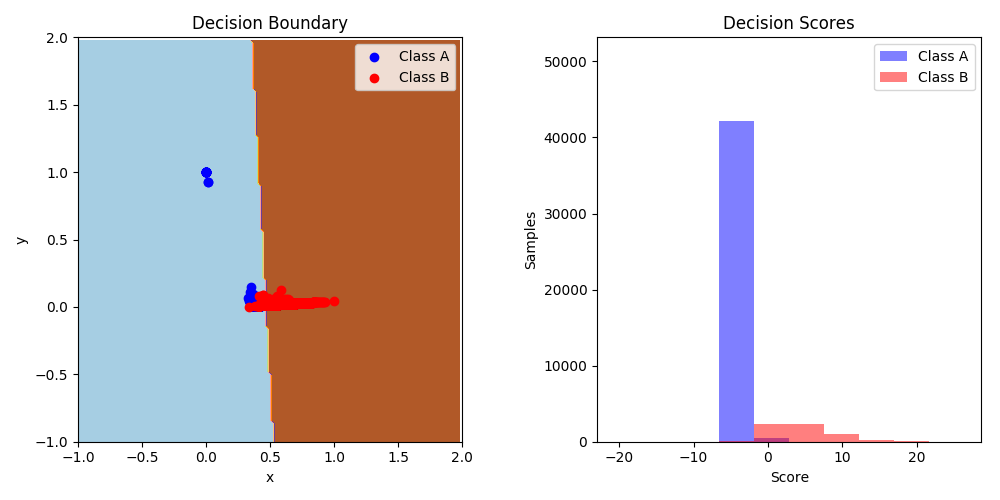
\includegraphics[width=1.0\textwidth]{../lr.png}
\caption{Logistic Regression}
\label{fig:lr}
\end{figure}
\begin{figure}[htbp]
\centering
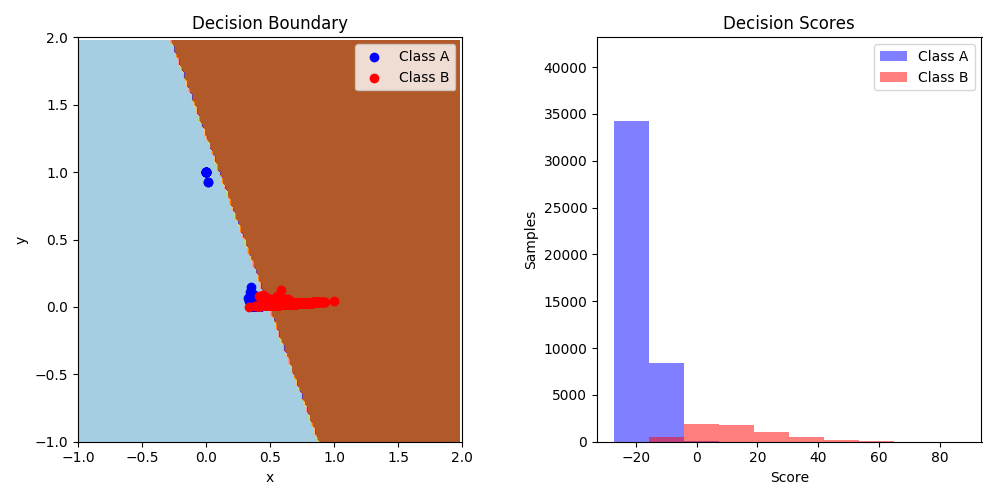
\includegraphics[width=1.0\textwidth]{../lda.png}
\caption{Linear Discriminant Analysis}
\label{fig:lda}
\end{figure}
\begin{figure}[htbp]
\centering
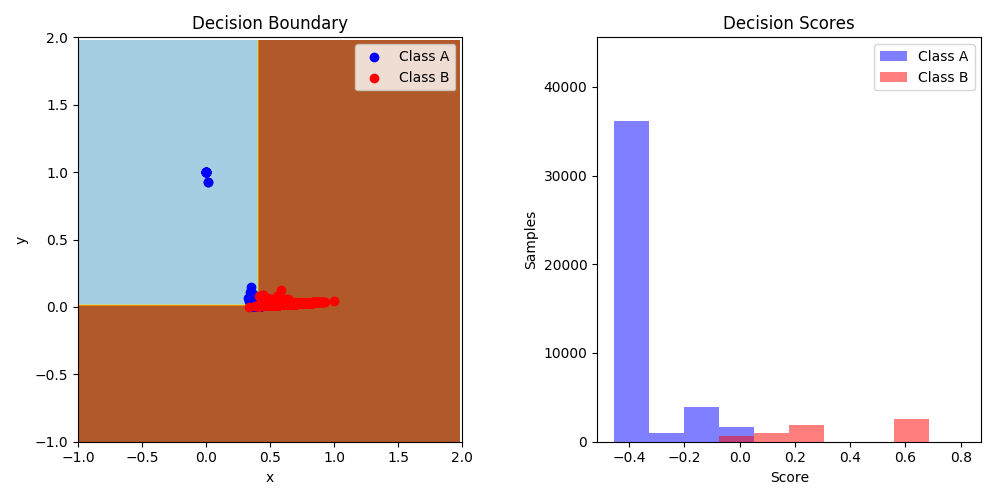
\includegraphics[width=1.0\textwidth]{../adaboost.png}
\caption{AdaBoost}
\label{fig:ada}
\end{figure}
\begin{figure}[htbp]
\centering
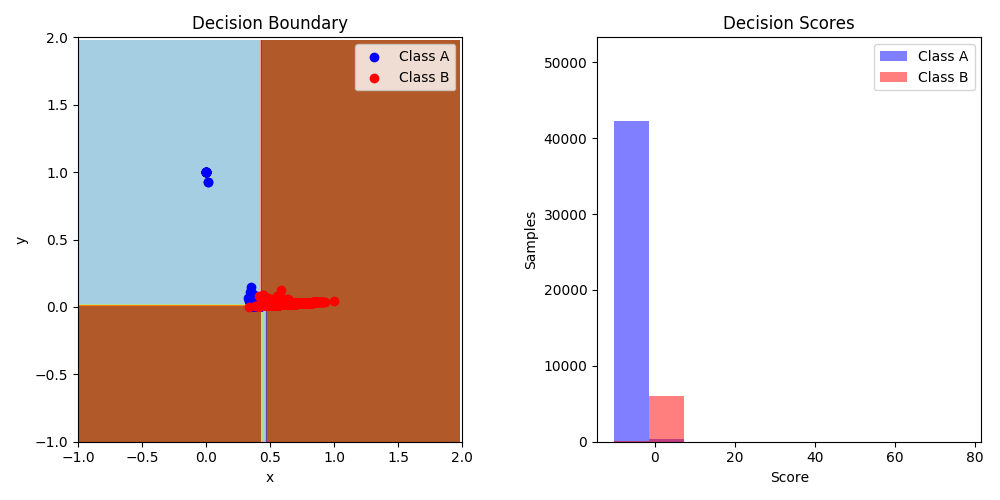
\includegraphics[width=1.0\textwidth]{../gradboost.png}
\caption{Gradient Boost(sklearn)}
\label{fig:grad}
\end{figure}
\\
前两者的判决边界像一条线,后两者的判决边界更复杂一些。分类结果如下:\\
\\
\begin{tabular}{l|r|r|r}
  \hline
  &Precision&Recall&F1-score\\
  \hline
  Logistic Regression$^{\ref{fig:lr}}$& 1.00&0.88&0.94\\
  \hline
  Linear Discriminant Analysis$^{\ref{fig:lda}}$&1.00&0.81&0.90\\
  \hline
  AdaBoost$^{\ref{fig:ada}}$&0.97&0.96&0.97\\
  \hline
  Gradient Boost(sklearn)$^{\ref{fig:grad}}$&0.98&0.96&0.97\\
  \hline
\end{tabular}
\\
\\
可以发现前两个分类器的效果不如后两个。从可视化的结果上也可以看出,
前两个分类器判决边界一刀切,缺了一些灵活性,不如后两者效果好。
\newpage
\subsection{聚类结果可视化}
使用 K-means(random) 聚类,将结果可视化。效果比预期要差,看不到太多明显的类别。AMI 0.1867, 
NMI 0.1993。\\
\begin{figure}[htbp]
\centering
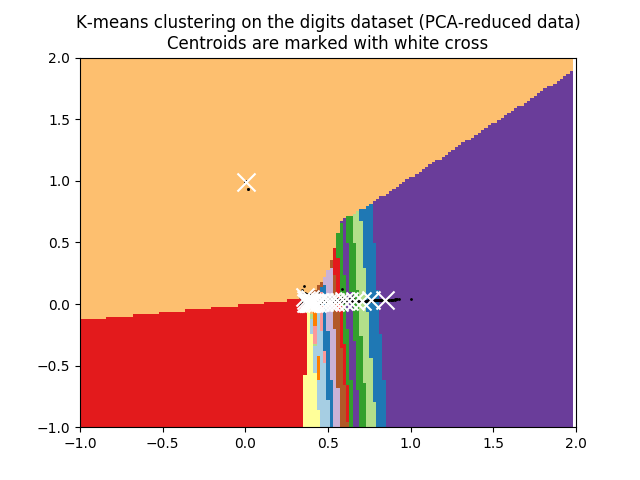
\includegraphics[width=1.0\textwidth]{../kmeans.png}
\caption{K-means}
\label{fig:K-means}
\end{figure}

\begin{figure}[htbp]
\centering
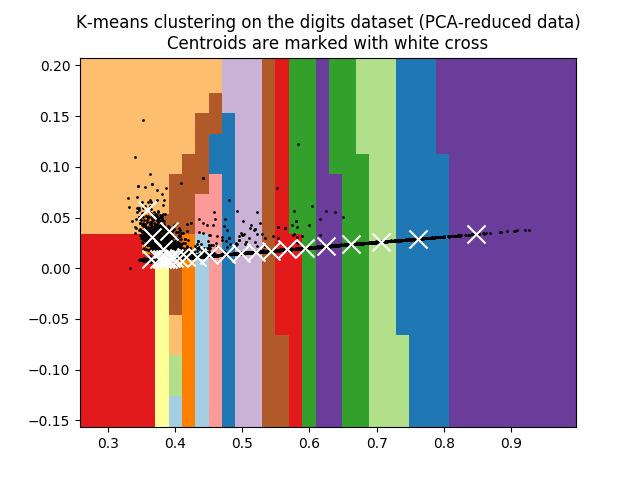
\includegraphics[width=1.0\textwidth]{../kmeans_2.png}
\caption{局部放大}
\label{fig:K-means_2}
\end{figure}

\begin{figure}[htbp]
\centering
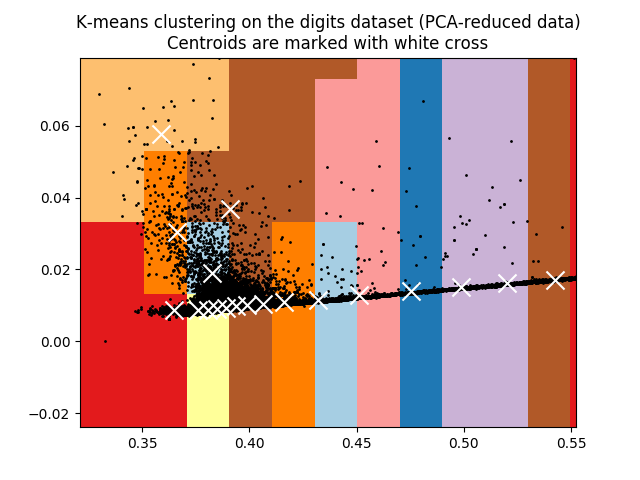
\includegraphics[width=1.0\textwidth]{../kmeans_3.png}
\caption{局部放大}
\label{fig:K-means_3}
\end{figure}




\end{document}  

